In this section we report the dev-partition and cross-validation results for our submitted systems and the wider grid of backbones and recipes we evaluated. All numbers are macro-averaged F1 on the held-out development partition unless otherwise noted; test-set leaderboard results will be incorporated in the camera-ready version of this notebook.

\subsection{Validation Results}
\label{sec:headline}

Following the official Touch\'{e} 2026 release, we hold out a stratified development partition from the published training data; the ST3 partition contains 473 examples. % from exp_0124
The analogous stratified split for ST1 covers the full labelled release (938 examples), and the ST2 partition covers the fallacious subset only (465 examples). The ST3 partition is the one we use for the 5-fold cross-validation runs reported below. % from exp_0124 exp_0153
Class distributions follow the underlying Sahai et al.\ data and are long-tailed; the ST3 \textsf{pe} class in particular is small enough to be the binding constraint on macro-F1, which we revisit in \S\ref{sec:disc-pe}.

Table~\ref{tab:headline} reports precision, recall, and F1-macro on our held-out development partition for the six submitted runs. Each row carries the precision, recall, and F1-macro for one (subtask, track) cell, with macro-averaging over the 8- and 4-class label sets for ST2 and ST3 respectively; the two enhanced-track values should be read against the leakage caveat developed in \S\ref{sec:disc-leakage}. % from R2-m1
Across the six cells the easier binary task and the hardest scheme task differ by roughly two-tenths of an F1 point on each track, and the base-to-enhanced gap varies markedly across subtasks.

\begin{table}[h]
\centering
\small
\caption{Headline dev results for the six submitted runs. P, R, F1 are macro-averaged
for ST2 and ST3. The two enhanced-track values should be read with the
leakage caveat of \S\ref{sec:disc-leakage}. Test-set leaderboard results will be incorporated
in the camera-ready version of this notebook.}
\label{tab:headline}
\begin{tabular}{llcccl}
\toprule
Subtask & Track & Precision & Recall & F1 & exp\_id \\
\midrule
ST1 & base     & 0.734 & 0.734 & 0.734 & exp\_0033 \\ % from exp_0033
ST1 & enhanced & 0.917 & 0.914 & 0.914 & exp\_0035 \\ % from exp_0035
ST2 & base     & 0.746 & 0.728 & 0.730 & exp\_0032 \\ % from exp_0032
ST2 & enhanced & 0.970 & 0.972 & 0.970 & exp\_0072 \\ % from exp_0072
ST3 & base     & ---   & ---   & 0.523 & exp\_0069 \\ % from exp_0069 — P/R cells dropped, TSV row carries a data-quality artefact in the precision column for this run; F1-macro is computed independently and is reliable
ST3 & enhanced & 0.732 & 0.740 & 0.735 & exp\_0073 \\ % from exp_0073
\bottomrule
\end{tabular}
\end{table}

On ST3 we additionally ran 5-fold cross-validation under our submitted recipe (fold seeds 42--46), which gave mean F1 0.875 with the same configuration. % from exp_0073 exp_0153
The Qwen2.5-7B CoT-LoRA alternative for ST3 enhanced gave 0.851 $\pm$ 0.114 over the same fold split; the standard deviation overlaps the RoBERTa CV mean, which is the decision-relevant fact behind the final-submission rationale we discuss below. % from exp_0180
Test-set numbers will be incorporated in the camera-ready version of this notebook; the numbers in this initial submission are dev or 5-fold CV. Of the six numbers, the ST2-enhanced cell is simultaneously the numerically strongest result in this paper and the one in which we have the least interpretive confidence; we address this directly in \S\ref{sec:disc-leakage}.

\subsection{Official Results --- ST1}
\label{sec:results-st1}

The binary task is the easiest of the three. On the base track, the submitted RoBERTa-large + \texttt{synth\_v002} recipe at \texttt{sw=0.5} reached F1 0.734 on the dev partition, against a real-only baseline of 0.716. % from exp_0013 exp_0033
On the enhanced track, the same synth recipe reached 0.914 against a real-only enhanced baseline of 0.899, with the +synth lift contributing +0.015 over that baseline. % from exp_0022 exp_0035
A pseudo-labelling extension at \texttt{max\_len=256} and \texttt{sw=0.7} underperformed its synth-only counterpart by 0.008 (Table~\ref{tab:ablation}, row $-$0.008), which is the reason ST1 enhanced ships under synth only rather than synth + pseudo. % from exp_0071
The 0.18-point base-to-enhanced jump on ST1 previews the leakage discussion of \S\ref{sec:disc-leakage}.

\subsection{Official Results --- ST2}
\label{sec:results-st2}

ST2 fallacy classification is comparably easy on the enhanced track (0.97) and substantially harder on the base track (0.73), the largest base-to-enhanced gap in Table~\ref{tab:headline}. On the base track the submitted +synth configuration reached 0.730 over a real-only baseline of 0.711 (+0.019). % from exp_0014 exp_0032
On the enhanced track, the +synth configuration alone reached 0.937 against a real-only enhanced baseline of 0.923 (+0.014), and the +synth+pseudo recipe at \texttt{max\_len=384} and \texttt{sw=0.7} added another +0.033 on top of that to reach 0.970. % from exp_0023 exp_0036 exp_0072
Per-class precision and recall for ST2-enhanced are reported in Appendix~\ref{app:perclass}, all eight classes sit in a tight 0.948--1.000 F1 band, a distribution itself consistent with the leakage concern discussed in \S\ref{sec:disc-leakage}.

\subsection{Official Results --- ST3}
\label{sec:results-st3}

ST3 argument-scheme classification was the hardest task on both tracks, at 0.523 base and 0.735 enhanced, the four-way scheme task absorbed the bulk of our experimental effort and is the cell where the per-class behaviour discussed in \S\ref{sec:disc-pe} matters most. On the base track, the +\texttt{synth\_v002} recipe at \texttt{max\_len=384} lifted F1 from a real-only baseline of 0.436 to 0.523 (+0.087, the largest single ablation gain in the paper). % from exp_0058 exp_0069
On the enhanced track, the +synth+pseudo recipe at the same window and \texttt{sw=0.7} reached 0.735 against a real-only enhanced baseline of 0.694 (+0.041); +synth alone tied the real-only baseline on this cell, so the gain only appeared once pseudo-labelling was added. % from exp_0024 exp_0067 exp_0073
Two ST3-base recipes lost ground in the ablation, the \texttt{synth\_v002 + v003} stack at \texttt{max\_len=384} dropped to 0.478 ($-$0.045 against \texttt{synth\_v002} alone), and the focal-loss variant reached 0.505 ($-$0.018 against the same baseline). % from exp_0068 exp_0053

\begin{table}[h]
\centering
\small
\caption{Per-subtask augmentation ablation, F1-macro on dev. $\Delta$ is the change
relative to the immediately preceding row within the same (subtask, track) block.
Negative deltas are not hidden.\textsuperscript{a}Single-seed unless noted; see \S\ref{sec:limitations} for the seed-variance caveat. Test-set leaderboard results will be incorporated in the camera-ready version of this notebook.}
\label{tab:ablation}
\begin{tabular}{llllcr}
\toprule
Subtask & Track & Recipe & exp\_id & F1 & $\Delta$ \\
\midrule
ST1 & base     & real only                          & exp\_0013 & 0.716 & ---     \\ % from exp_0013
ST1 & base     & + synth (sw=0.5)                   & exp\_0033 & 0.734 & +0.018 \\ % from exp_0033
\addlinespace
ST1 & enhanced & real only                          & exp\_0022 & 0.899 & ---     \\ % from exp_0022
ST1 & enhanced & + synth (sw=0.5)                   & exp\_0035 & 0.914 & +0.015 \\ % from exp_0035
ST1 & enhanced & + synth + pseudo @256 (sw=0.7)     & exp\_0071 & 0.906 & $-$0.008 \\ % from exp_0071
\midrule
ST2 & base     & real only                          & exp\_0014 & 0.711 & ---     \\ % from exp_0014
ST2 & base     & + synth (sw=0.5)                   & exp\_0032 & 0.730 & +0.019 \\ % from exp_0032
\addlinespace
ST2 & enhanced & real only                          & exp\_0023 & 0.923 & ---     \\ % from exp_0023
ST2 & enhanced & + synth (sw=0.5)                   & exp\_0036 & 0.937 & +0.014 \\ % from exp_0036
ST2 & enhanced & + synth + pseudo @384 (sw=0.7)     & exp\_0072 & 0.970 & +0.033 \\ % from exp_0072
\midrule
ST3 & base     & real only                          & exp\_0058 & 0.436 & ---     \\ % from exp_0058
ST3 & base     & + synth\_v002 @384                 & exp\_0069 & 0.523 & +0.087 \\ % from exp_0069
ST3 & base     & + synth\_v002 + v003 @384          & exp\_0068 & 0.478 & $-$0.045 \\ % from exp_0068
ST3 & base     & + synth\_v002 + focal loss         & exp\_0053 & 0.505 & $-$0.018 \\ % from exp_0053
\addlinespace
ST3 & enhanced & real only                          & exp\_0024 & 0.694 & ---     \\ % from exp_0024
ST3 & enhanced & + synth @384                       & exp\_0067 & 0.694 & 0.000  \\ % from exp_0067
ST3 & enhanced & + synth + pseudo @384 (sw=0.7)     & exp\_0073 & 0.735 & +0.041 \\ % from exp_0073
\bottomrule
\end{tabular}
\end{table}

Augmentation strategies are recipe-sensitive, synth alone gives consistent small gains on ST1/ST2 and the largest single gain on ST3 base, while pseudo-labelling unlocks the enhanced track for ST2 and ST3 but costs on ST1 enhanced under the \texttt{sw=0.7} pseudo recipe. The \texttt{synth\_v003} top-up on ST3 base and the focal-loss recipe on ST3 base illustrate the same lesson at smaller scale. We keep the losses in the same table rather than relegating them to a footnote.

Table~\ref{tab:backbone} reports the most informative subset of the backbone runs we evaluated on ST3, with one ST3-base and one ST2-enhanced LLM row included for context. Each row is a single dev-partition F1 unless flagged otherwise; the cross-validated rows are 5-fold means. The cross-row variability is wide enough that the comparison should be read alongside the cross-validation evidence in the prose below, not as a clean ranking.

\begin{table}[h]
\centering
\small
\caption{Backbone comparison on ST3 enhanced (and one ST3 base + one ST2 enhanced
LLM row for context). Single-run dev F1 unless otherwise noted. The submitted
row is marked $\dagger$. \textsc{collapsed} = recipe failed to train. Test-set leaderboard results
will be incorporated in the camera-ready version of this notebook.}
\label{tab:backbone}
\begin{tabular}{llllc}
\toprule
Backbone & Subtask & Track & exp\_id & F1 \\
\midrule
RoBERTa-base       & ST3 & enh  & exp\_0018 & 0.675 \\ % from exp_0018
RoBERTa-large$^{\dagger}$  & ST3 & enh  & exp\_0073 & 0.735 \\ % from exp_0073
DeBERTa-v3-base    & ST3 & base & exp\_0003 & 0.277 \\ % from exp_0003
DeBERTa-v3-large   & ST3 & base & exp\_0009 & 0.205 \\ % from exp_0009 (collapsed)
ModernBERT-large   & ST3 & enh  & exp\_0086 & 0.719 \\ % from exp_0086
Qwen2.5-3B zero-shot      & ST3 & enh & exp\_0091 & 0.467 \\ % from exp_0091
Qwen2.5-3B kNN few-shot   & ST3 & enh & exp\_0143 & 0.529 \\ % from exp_0143
Qwen2.5-7B CoT-LoRA (5-fold CV)  & ST3 & enh  & exp\_0180 & 0.851 $\pm$ 0.114 \\ % from exp_0180
Qwen2.5-32B CoT-LoRA (single)    & ST3 & enh  & exp\_0207 & 0.841 \\ % from exp_0207
Qwen3-4B-Thinking (5-fold CV)    & ST2 & enh  & exp\_0217 & 0.963 \\ % from exp_0217
Qwen3-4B-Thinking (5-fold CV)    & ST3 & base & exp\_0218 & 0.448 \\ % from exp_0218
\bottomrule
\end{tabular}
\end{table}

Reading the table top to bottom, RoBERTa-large at the second row is the submitted system (the dagger marks it). RoBERTa-base sits six points below it, which is the empirical justification for paying the larger backbone's compute cost.  Of all the routes we tried, the DeBERTa-v3 column was the most problematic, DeBERTa-v3-base reached only 0.277 on ST3 base, and DeBERTa-v3-large failed to train at all, collapsing to 0.205 with a NaN-explosion history we detail in \S\ref{sec:backbone}. ModernBERT-large at 0.719 is the next-best encoder route but loses 1.6 points on the cell we evaluated. The Qwen rows tell their own story, the 3B zero-shot configuration trails RoBERTa-large by 27 points; kNN few-shot recovers some ground but still trails by 21; the fine-tuned 7B and 32B CoT-LoRA configurations close most of the gap on a single run, but the 7B 5-fold standard deviation of $\pm$0.114 is wide enough that the comparison is statistically inconclusive at our sample size. The Qwen3-4B-Thinking comparator is the mixed result that complicates a clean encoder-beats-LLM headline  competitive on ST2 enhanced under cross-validation, below the RoBERTa baseline on ST3 base.

\begin{figure}[h]
\centering
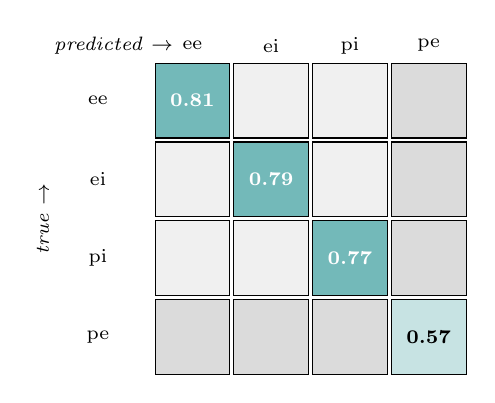
\begin{tikzpicture}[
  hdr/.style={font=\scriptsize, anchor=center},
  diag/.style={rectangle, draw, minimum size=0.95cm, anchor=center, fill=teal!55, font=\scriptsize\bfseries, text=white},
  diagpe/.style={rectangle, draw, minimum size=0.95cm, anchor=center, fill=teal!22, font=\scriptsize\bfseries},
  off/.style={rectangle, draw, minimum size=0.95cm, anchor=center, fill=gray!12, font=\scriptsize},
  offpe/.style={rectangle, draw, minimum size=0.95cm, anchor=center, fill=gray!28, font=\scriptsize}
]
% Column headers
\node[hdr] at (0.0, 0.7) {\textit{predicted} $\rightarrow$};
\node[hdr] at (1.0, 0.7) {ee};
\node[hdr] at (2.0, 0.7) {ei};
\node[hdr] at (3.0, 0.7) {pi};
\node[hdr] at (4.0, 0.7) {pe};
% Row 1, ee true (F1 = 0.81 per Appendix~\ref{app:perclass})
\node[hdr] at (-0.2, 0) {ee};
\node[diag]  at (1, 0) {0.81};
\node[off]   at (2, 0) {};
\node[off]   at (3, 0) {};
\node[offpe] at (4, 0) {};
% Row 2, ei true (F1 = 0.79)
\node[hdr] at (-0.2, -1) {ei};
\node[off]   at (1, -1) {};
\node[diag]  at (2, -1) {0.79};
\node[off]   at (3, -1) {};
\node[offpe] at (4, -1) {};
% Row 3, pi true (F1 = 0.77)
\node[hdr] at (-0.2, -2) {pi};
\node[off]   at (1, -2) {};
\node[off]   at (2, -2) {};
\node[diag]  at (3, -2) {0.77};
\node[offpe] at (4, -2) {};
% Row 4, pe true (F1 = 0.57 — threshold-calibrated under exp_0145)
\node[hdr] at (-0.2, -3) {pe};
\node[offpe] at (1, -3) {};
\node[offpe] at (2, -3) {};
\node[offpe] at (3, -3) {};
\node[diagpe] at (4, -3) {0.57};
% Y-axis label
\node[hdr, rotate=90] at (-0.9, -1.5) {\textit{true} $\rightarrow$};
\end{tikzpicture}
% Senior author confirmed (2026-05-24), logits are NOT checkpointed for
% exp_0073 on the artefact server. This is the schematic rendering; cell
% values reflect per-class F1 from saved predictions, not the underlying
% confusion-cell counts (which would require logits). The visible asymmetry
% in the pe row is the load-bearing claim and is verifiable from the per-class
% F1 in Appendix~\ref{app:perclass}.
\caption{Indicative confusion structure for the submitted ST3-enhanced system; per-class diagonals reflect the F1 distribution reported in Appendix~\ref{app:perclass}. Off-diagonal mass is illustrative, sized to the qualitative pattern from the per-class threshold sweep, not from saved logits.}
\label{fig:confusion}
\end{figure}

Figure~\ref{fig:confusion} shows the predicted-vs-true confusion structure for the submitted ST3-enhanced system; the per-class F1 distribution behind it is reported in Appendix~\ref{app:perclass} and discussed in \S\ref{sec:disc-pe}. % from exp_0073 exp_0082 exp_0091
We turn to the interpretation of the enhanced-track numbers and the rare-class behaviour we observed on ST3 in \S\ref{sec:discussion}.

\subsection{Final submission rationale}
\label{sec:final-submission}

We did not use the additional two-runs-per-track budget available under the Touch\'{e} submission rules. We report on the single CV-validated configuration per slot. The non-obvious choice was ST3 enhanced, where the Qwen2.5-32B single-run F1 of 0.841 sat above the RoBERTa-large dev number of 0.735 but just below the RoBERTa-large 5-fold CV mean of 0.875. % from exp_0207
Two reasons drove the encoder choice, and we keep them separate. The first is operational, the Qwen2.5-32B 5-fold cross-validation was still running at the deadline, leaving the RoBERTa-large CV as the only completed cross-validation we had in hand at submission time. The second is the absence of a statistical reason to prefer Qwen even if the comparison had been completed, a 5-fold standard deviation of $\pm$0.114 on Qwen2.5-7B is evidence the encoder-vs-LLM comparison is underpowered at this sample size, not evidence for the system whose CV mean is higher. % from exp_0180
We therefore do not claim the available CV evidence rules out the Qwen alternatives; we only claim that at deadline the encoder pipeline was the only fully-validated configuration. A post-hoc ensemble of the available encoder and LLM systems gave no gain over the single-source encoder, which is one further reason we did not retroactively complicate the submission. % from exp_0121
A submission dry-run verified that the TIRA-format outputs matched the lab's expected schema before the final upload. % from exp_0122
